\documentclass[11pt,a4paper,oldfontcommands]{memoir}
\usepackage[utf8]{inputenc}
\usepackage[T1]{fontenc}
\usepackage{microtype}
\usepackage[dvips]{graphicx}
\usepackage{xcolor}
\usepackage{bookman}
\usepackage{graphicx,xcolor}
\usepackage[usestackEOL]{stackengine}
\usepackage[percent]{overpic}


\usepackage[
breaklinks=true,colorlinks=true,
%linkcolor=blue,urlcolor=blue,citecolor=blue,% PDF VIEW
linkcolor=black,urlcolor=black,citecolor=black,% PRINT
bookmarks=true,bookmarksopenlevel=2]{hyperref}

\usepackage{geometry}
% PDF VIEW
% \geometry{total={210mm,297mm},
% left=25mm,right=25mm,%
% bindingoffset=0mm, top=25mm,bottom=25mm}
% PRINT
\geometry{total={210mm,297mm},
left=20mm,right=20mm,
bindingoffset=10mm, top=25mm,bottom=25mm}

\OnehalfSpacing
%\linespread{1.3}

%%% CHAPTER'S STYLE
\chapterstyle{ell}
%\chapterstyle{ger}
%\chapterstyle{madsen}
%\chapterstyle{ell}
%%% STYLE OF SECTIONS, SUBSECTIONS, AND SUBSUBSECTIONS
\setsecheadstyle{\Large\bfseries\sffamily\raggedright}
\setsubsecheadstyle{\large\bfseries\sffamily\raggedright}
\setsubsubsecheadstyle{\bfseries\sffamily\raggedright}


%%% STYLE OF PAGES NUMBERING
%\pagestyle{companion}\nouppercaseheads 
%\pagestyle{headings}
%\pagestyle{Ruled}
\pagestyle{plain}
\makepagestyle{plain}
\makeevenfoot{plain}{\thepage}{}{}
\makeoddfoot{plain}{}{}{\thepage}
\makeevenhead{plain}{}{}{}
\makeoddhead{plain}{}{}{}


\maxsecnumdepth{subsection} % chapters, sections, and subsections are numbered
\maxtocdepth{subsection} % chapters, sections, and subsections are in the Table of Contents


%%%---%%%---%%%---%%%---%%%---%%%---%%%---%%%---%%%---%%%---%%%---%%%---%%%
\begin{document}

%%%---%%%---%%%---%%%---%%%---%%%---%%%---%%%---%%%---%%%---%%%---%%%---%%%
%   TITLEPAGE
%
%   due to variety of titlepage schemes it is probably better to make titlepage manually
%
%%%---%%%---%%%---%%%---%%%---%%%---%%%---%%%---%%%---%%%---%%%---%%%---%%%
\thispagestyle{empty}

{%%%
\sffamily

\centering
\Large

~\vspace{\fill}

{\huge 

\includegraphics{img/logo.png}\\
TOPLIS
}

\vspace{2.5cm}

{\LARGE
TopSky plugin for Portugal vACC
}

\vspace{3.5cm}

User Manual\\
Version 2.0\\

\vspace{\fill}

October 2022

%%%
}%%%

\cleardoublepage
%%%---%%%---%%%---%%%---%%%---%%%---%%%---%%%---%%%---%%%---%%%---%%%---%%%
%%%---%%%---%%%---%%%---%%%---%%%---%%%---%%%---%%%---%%%---%%%---%%%---%%%

\tableofcontents*

\clearpage

%%%---%%%---%%%---%%%---%%%---%%%---%%%---%%%---%%%---%%%---%%%---%%%---%%%
%%%---%%%---%%%---%%%---%%%---%%%---%%%---%%%---%%%---%%%---%%%---%%%---%%%

\chapter{Introduction}

\section{Disclaimer}
Although - as its name suggests - the plugin is based on TOPLIS and the TopSky ATM system, it is in no way affiliated with or endorsed by Thales Group or NAV Portugal. Similarities between plugin features and the real system are not entirely coincidental, but the plugin can not be used as a real world training aid. ~\cite{git}\\

\section{Foreword}
EuroScope, a controller client developed by Gergely Csernák for the VATSIM network, was first released for public use in September 2007. One of the biggest changes in version 3.1 was the possibility for the user community to customize the program to an even higher degree than was possible before by writing their own plugins that can be used to alter the way information is presented and even create completely new functionality into the program. This allowed creating very detailed simulations of all kinds of ATC systems without making the main program overly complex. Version 3.2 expands on these possibilities, making it possible to create even better plugins.
The TopSky plugin (a.k.a. The Plugin Formerly Known As “EUROCAT 2000 E”) started out as a very small project to create a couple of customized aircraft tag items, but as more information about the real system and the possibilities with the plugin development became available, it slowly grew to include an almost complete set of tag items, tag menus, graphical elements on the radar display and some additional functionality.

\chapter{System Description}
\section{Main Window}
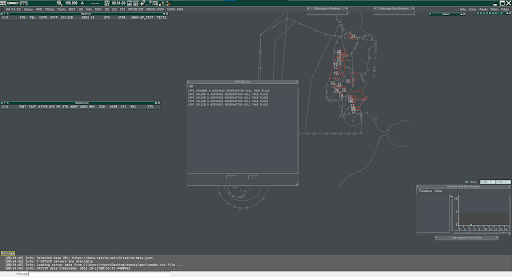
\includegraphics[width=15cm, keepaspectratio]{img/mainwindow.png}\\
Euroscope should load with some preplaced windows similar to the above configuration\\

Screen resolutions other than 1920x1080 will yield different results. Larger resolutions will bring preplaced windows towards the left and middle, while smaller resolutions may potentially place windows outside the screen. It is recommended for users experiencing difficulties related to their screen size to experiment and create custom settings in the TopSkySettingsLocal file containing revised window placements adjusted for their own screen. Refer to \texttt{\detokenize{TopSky_Developer_Guide_Settings.xlsx}} for available settings.\\

\section{Global Menu}

\includegraphics{img/globalmenu.png}\\
The Global Menu is located on the top edge of the radar screen. It displays the current UTC time and contains a number of submenus which are explained below.

\subsection{Setup}
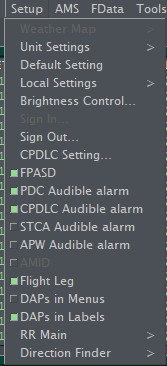
\includegraphics{img/Setup.png}\\
Setup Menu allows for various adjustments. Each position will load its defined settings based on the active Primary Frequency.\\ 
Most used options are CPDLC Setting for CPDLC operations and Default Setting to reset options.\\

\begin{tabular}{p{5cm}p{10cm}}
- Unit Settings > & Opens the Unit Settings submenu
\\- Default Setting & Resets all settings to their default values (keeps login callsign specific ones if they are active at the time). When clicked, a confirmation window will open, asking to confirm the reset.
\\- Local Settings > & Opens the Local Settings submenu
\\- Brightness Control > & Opens the Brightness Control Window
\\- Sign In… & Loads personal settings. The settings are specified in the \texttt{\detokenize{TopSkySettingsLocal.txt}} data file. When clicked, a confirmation window will open, asking to confirm the settings change.
\\- Sign Out… & Clears any personal settings and resets all settings to their default values. When clicked, a confirmation window will open, asking to confirm the settings change.
\\- CPDLC Setting… & Opens the CPDLC Setting Window
\\- FPASD & Toggles on/off the display of flight plan tracks
\\- PDC Audible alarm & Toggles on/off playing a sound for received PDC messages
\\- CPDLC Audible alarm & Toggles on/off playing a sound for received CPDLC messages
\\- STCA Audible alarm & Toggles on/off playing a sound for STCA alerts
\\- APW Audible alarm & Toggles on/off playing a sound for APW alerts
\\- AMID & Not implemented
\\- Flight Leg & Toggles on/off the automatic display of the Flight Leg for a specified time when a track becomes assumed
\\- DAPs in Menus & Toggles on/off the display of DAPs in menus
\\- DAPs in Labels & Toggles on/off the display of DAPs in track labels
\\- RR Main > & Opens the RR Main submenu
\\- Direction Finder > & Opens the Direction Finder submenu
  \end{tabular}

\subsection{AMS (Airspace Management System)}
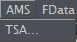
\includegraphics{img/AMS.png}\\
Used to access \textit{\titleref{menu:tsa}}.

\subsection{FData menu}
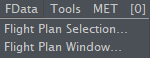
\includegraphics{img/FData.png}\\
Used to access \textit{\titleref{menu:fpsel}} and \textit{\titleref{menu:fpwin}}.

\subsection{Tools menu}
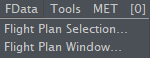
\includegraphics{img/FData.png}\\
\begin{tabular}{p{5cm}p{10cm}}
\\- Flight Plan Lists > & Opens the Flight Plan Lists submenu
\\- CARD… & Opens the Conflict And Risk Display
\\- SAP… & Opens the Segregated Area Probe Window
\\- Vertical Aid Window… & Opens the Vertical Aid Window
\\- Message In… & Opens the Message In Window
\\- Message Out… & Opens the Message Out Window
\\- CPDLC > & Opens the CPDLC submenu
\\- LAT/LONG… & Opens the Cursor Lat/Long Window
\end{tabular}

\section{NOTAM List}
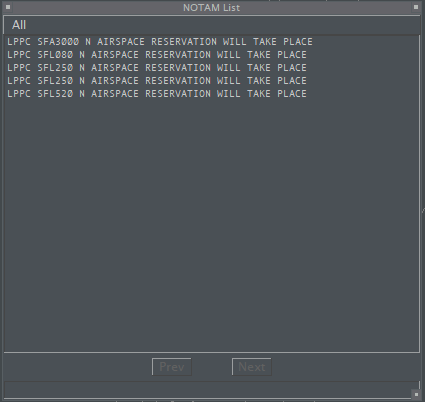
\includegraphics{img/notamlist.png}\\
The NOTAM List is automatically displayed at startup in order to fetch the current FUA. It may be closed after loading.\\

\section{TSA (Temporary Segregated Areas) Menu}
\label{menu:tsa}
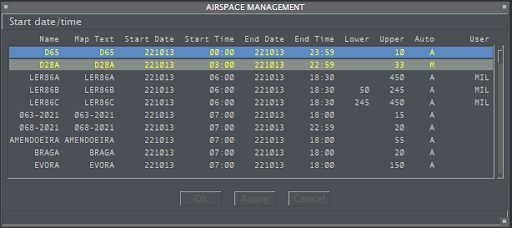
\includegraphics{img/tsa.png}\\
This window is used for the activation and deactivation of the areas for the APW and SAP functionality. Each area can have a start time and/or an end time defined for its activation, or it can be activated without any time limits, making it active until deactivated manually. Additionally, lower and upper altitude limits are given. An area can have activation schedules defined in the area data file. Such areas will be automatically activated as long as their “Auto” option is selected ( “A” in the “Auto” column). The “Auto” option cannot be selected for areas that don’t have an activation schedule defined in the area data file.

Dates will be shown in the format “yymmdd” and times in “hh:mm” and they must be entered in the same format. Entering an empty string for a date will clear it and the related time value and vice versa. When entering a time or date value to an empty field, the other value is automatically set to the current time/date value. Entering an empty string to the Map Text, Lower or Upper fields will reset the value to the default one from the data file.

Altitudes are shown in hundreds of feet if at or below the transition altitude, otherwise in flight levels. They must be entered in the same format.

An area’s activation status can be inactive, pre-active or active. A pre-active area is an area that will become active within 30 minutes and is shown in yellow text on a gray background. An active area is shown with yellow text on a blue background. The APW system will not alert for a pre-active area, but for the SAP system a pre-active area is considered as being active.

The mouse click areas of the Airspace Management Window:
\begin{itemize}[\textbullet] 
    \item Sorting option text (e.g. “Start date/time”) Opens a pop-up menu to select a sorting option for the list 
    \item Right-click to open an area pop-up menu
    \item Other fields Left-click to edit field (when edit function active)
    \item “Ok” button Applies the changes, closes the window
    \item “Apply” button Applies the changes
    \item “Cancel” button Cancels the changes 
\end{itemize}

The sorting pop-up menu contains the following items:
\begin{itemize}[\textbullet] 
    \item Start Date Sorts based on the Start Date/Time, earliest first
    \item Name Sorts alphabetically based on the Name field
    \item Map Text Sorts alphabetically based on the Map Text field 
\end{itemize}
With the area pop-up menu opened, the area text row background changes to black. The menu contains the following items:
\begin{itemize}[\textbullet] 
    \item ACTIVATE Clears any activation times and activates the area
    \item DEACTIVATE Clears any activation times and deactivates the area
    \item AUTO If an activation schedule is found in the area data file, sets the
    \item area to be activated automatically
    \item VALIDATE Not implemented
    \item EDIT Allows to change the area parameters
    \item COPY Not implemented
    \item DELETE Clears any activation times, returns label and altitude limits to their default values and deactivates the area
\end{itemize}
After any selection from the pop-up menu, “Ok”, “Apply” or “Cancel” must be selected to apply or cancel the selection. 

Preactive and active areas are displayed on the radar screen. The area border is drawn using a predefined color and it may be filled as well. A predefined text label may also be displayed, showing information about the area. A very small “+” symbol will be drawn at that location. By holding the left mouse button down on that symbol, a full area label will be displayed, showing:

\begin{center}
        Name\\ 
        Map text\\
        Upper level limit\\
        Start time --------- End time\\
        Lower level limit\\ime in minutes until the area becomes active
\end{center}

\appendix

\chapter{Additional}
Lorem ipsum dolor sit amet, consectetur adipiscing elit, sed do eiusmod tempor incididunt ut labore et dolore magna aliqua. Ut enim ad minim veniam, quis nostrud exercitation ullamco laboris nisi ut aliquip ex ea commodo consequat. Duis aute irure dolor in reprehenderit in voluptate velit esse cillum dolore eu fugiat nulla pariatur. Excepteur sint occaecat cupidatat non proident, sunt in culpa qui officia deserunt mollit anim id est laborum.


\bibliographystyle{unsrt}
\bibliography{refs}

\end{document}

